\documentclass[12pt,a4paper]{article}
\usepackage[a4paper,top=25mm,bottom=25mm,left=28mm,right=28mm]{geometry}
\usepackage[T1]{fontenc}
\usepackage[utf8]{inputenc}
\usepackage{times}
\usepackage{graphicx}
\usepackage{amssymb}
\usepackage{xcolor}
\usepackage{array}
\usepackage{setspace}
\usepackage{enumitem}
\usepackage{float}
\usepackage{tikz}
\usetikzlibrary{shapes.geometric, arrows.meta, positioning}
\usepackage[hidelinks]{hyperref}
\usepackage{chngcntr}
\counterwithin{figure}{section}
\onehalfspacing

\definecolor{boxblue}{RGB}{221,229,247}
\definecolor{okgreen}{RGB}{33,160,70}
\newcommand{\yes}{\textcolor{okgreen}{\checkmark}}

\setlength{\parindent}{0pt}
\setlength{\parskip}{6pt}

\begin{document}

% ===================== TITLE PAGE =====================
\thispagestyle{empty}
\begin{center}
    
\includegraphics[width=3.0cm]{puc_logo.png}\\[0.8cm]
    {\large PREMIER UNIVERSITY}\\[0.2cm]
    {\normalsize DEPARTMENT OF COMPUTER SCIENCE AND ENGINEERING}\\[0.5cm]
    {\itshape A Thesis Proposal On}\\[0.3cm]
    {\large \textbf{Explainable Cyberbullying Detection Using Deep Learning and Transformer Models with LIME}}\\[1.6cm]

    {\normalsize Submitted To:}\\[0.25cm]
    Tanni Dhoom\\
    Assistant Professor\\
    Department of Computer Science and Engineering\\[1.4cm]

    {\normalsize Submitted By:}\\[0.25cm]
    \textbf{Mohammad Asmual Hoque Yousha} (0222210005101121)\\
    \textbf{Md Mostafa Kamal Anna} (0222210005101129)\\[2.2cm]

    {\normalsize May, 2026}
\end{center}
\clearpage

\pagenumbering{roman}

% ===================== TABLE OF CONTENTS =====================
\renewcommand{\contentsname}{TABLE OF CONTENTS}
\begingroup
\makeatletter
\renewcommand{\@dotsep}{1.5}
\makeatother
\tableofcontents
\endgroup
\clearpage

% ===================== 1. INTRODUCTION =====================
\section{Introduction}
Social media platforms such as YouTube, Reddit, and Facebook now carry a huge share of everyday communication, and along with that scale comes a steady stream of hostile, threatening, and demeaning content. Cyberbullying, the repeated or aggressive targeting of a person through such content, has well-documented effects on the mental health of its victims, and the sheer volume of posts makes manual moderation impossible. Automatic detection has therefore become an active research problem. However, most existing detectors report only a label and give no reason for their decision, which makes them hard to trust and difficult to defend when a post is removed or a user is warned. This proposal sets out a project to build an accurate \emph{and} explainable cyberbullying detector that classifies English comments as Bullying or Not-Bullying, compares several deep learning models, and, as its main novelty, uses Local Interpretable Model-agnostic Explanations (LIME) to show the exact words behind every prediction.

% ===================== 2. OBJECTIVES =====================
\section{Objectives}
The project aims to build an AI-based system that detects cyberbullying in text and explains its decisions. Specifically, the project will:

\begin{itemize}[leftmargin=1.4em]
    \item Build a binary cyberbullying detector (Bullying vs Not-Bullying) on multi-platform English data.
    \item Implement and compare four models of increasing capability: TF--IDF Logistic Regression, LSTM, GRU, and a fine-tuned RoBERTa transformer.
    \item Collect data from YouTube, Reddit, and Facebook, and supplement it with the public Jigsaw toxic-comment corpus.
    \item Integrate LIME so that each prediction can be explained at the level of contributing words (the main contribution).
    \item Evaluate the models using accuracy, precision, recall, and F1-score, and compare the results against existing cyberbullying studies.
\end{itemize}

% ===================== 3. METHODOLOGY =====================
\section{Methodology}

\begin{figure}[H]
    \centering
    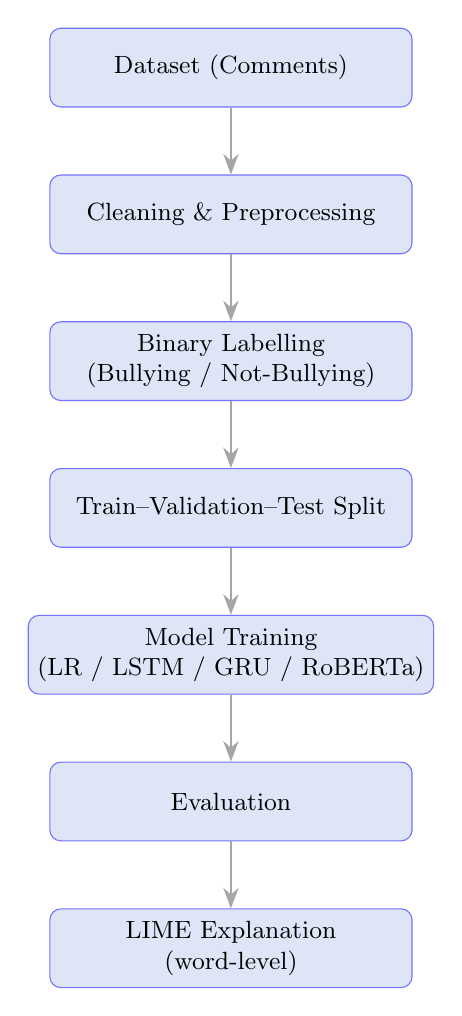
\begin{tikzpicture}[
        node distance=0.85cm,
        box/.style={rectangle, rounded corners=4pt, draw=blue!55, fill=boxblue, align=center,
                    minimum width=4.6cm, minimum height=1.0cm, font=\small},
        arr/.style={-{Stealth[length=2.6mm]}, thick, gray!70}
    ]
        \node[box] (d) {Dataset (Comments)};
        \node[box, below=of d] (c) {Cleaning \& Preprocessing};
        \node[box, below=of c] (l) {Binary Labelling\\(Bullying / Not-Bullying)};
        \node[box, below=of l] (s) {Train--Validation--Test Split};
        \node[box, below=of s] (m) {Model Training\\(LR / LSTM / GRU / RoBERTa)};
        \node[box, below=of m] (e) {Evaluation};
        \node[box, below=of e] (x) {LIME Explanation\\(word-level)};
        \draw[arr] (d)--(c); \draw[arr] (c)--(l); \draw[arr] (l)--(s);
        \draw[arr] (s)--(m); \draw[arr] (m)--(e); \draw[arr] (e)--(x);
    \end{tikzpicture}
    \caption{Overall workflow of the proposed explainable cyberbullying detection framework}
    \label{fig:workflow}
\end{figure}

\subsection{Dataset Collection and Preprocessing}
For this research, comments are collected from three social platforms, YouTube, Reddit, and Facebook, and supplemented with the publicly available Jigsaw Toxic Comment Classification Challenge corpus. The raw text is cleaned by removing URLs and normalising whitespace, after which near-duplicate comments are removed (deduplication is applied \emph{after} cleaning so that comments differing only by links or spacing are caught). Every comment is then reduced to a single binary label, Bullying or Not-Bullying.

\subsection{Model Development}
Four models spanning the classical-to-transformer range are developed: a TF--IDF Logistic Regression baseline, an LSTM and a GRU that model word order, and a fine-tuned RoBERTa transformer. LIME is applied on top of the best model to produce word-level explanations for individual predictions.

\subsection{Training and Validation}
The dataset is shuffled with a fixed random seed and divided into training, validation, and test sets using a stratified 70/15/15 split. Regularisation techniques such as dropout and early stopping are applied to the neural models to prevent overfitting, and the same split is reused for every model so that the comparison is fair.

\subsection{Evaluation}
The models are evaluated using accuracy, precision, recall, F1-score, and confusion matrices. To test generalisation, the full pipeline is also run on an external benchmark dataset, and the results are compared against existing studies in the literature.

\subsection{Implications and Applications}
(1) Verification and moderation of content on social networks and video-sharing platforms. (2) Protecting vulnerable users, such as teenagers, by surfacing harmful comments quickly. (3) Supporting human moderators with transparent, reviewable decisions rather than opaque labels.

\subsection{Challenges and Risks}
\textbf{Challenges:} (1) Sarcasm and irony are carried by tone rather than by any hostile word and are hard to detect. (2) Limited and imbalanced data can bias the models. (3) The meaning of ``bullying'' varies across datasets, making fair comparison difficult.\\
\textbf{Risks:} (1) False positives, where harmless comments are flagged, may erode user trust. (2) Detection may lag behind new forms of online abuse. (3) The current scope is English-only, limiting direct use on multilingual or code-mixed text.

% ===================== 4. GANTT CHART =====================
\section{Gantt Chart thesis timeline}
The project follows a structured six-month timeline running from May 2026 to October 2026. It begins in May with the \emph{Proposal and Literature Review}, where the problem is defined, objectives are set, and related work is surveyed, together with the start of \emph{Dataset Collection} from YouTube, Reddit, Facebook, and the Jigsaw corpus. In June, data collection continues alongside \emph{Data Preprocessing and Labelling}, where the text is cleaned, deduplicated, and reduced to a binary label, and the \emph{Model Development} phase begins. July and August cover \emph{Model Training and Validation} on the stratified split, \emph{Evaluation and Comparison} against prior work, and the \emph{LIME Explainability Integration} that adds word-level explanations to the best model. In September the team carries out the \emph{Error Analysis}, which examines where the model fails (most notably on sarcasm), and begins \emph{Report Writing}. Finally, October is devoted to \emph{Report Editing}, the \emph{Final Report and Review}, and the \emph{Submission and Defense}, where the completed work is presented before an academic panel. (Dates below are indicative and can be adjusted to the actual schedule.)

\begin{figure}[H]
\centering
\renewcommand{\arraystretch}{1.35}
\setlength{\tabcolsep}{5pt}
\small
\begin{tabular}{|p{5.2cm}|c|c|c|c|c|c|}
\hline
\textbf{Task} & \textbf{May} & \textbf{Jun} & \textbf{Jul} & \textbf{Aug} & \textbf{Sep} & \textbf{Oct} \\
 & '26 & '26 & '26 & '26 & '26 & '26 \\
\hline
1. Proposal \& Literature Review & \yes & & & & & \\ \hline
2. Dataset Collection & \yes & \yes & & & & \\ \hline
3. Preprocessing \& Labelling & & \yes & & & & \\ \hline
4. Model Development & & \yes & \yes & & & \\ \hline
5. Training \& Validation & & & \yes & \yes & & \\ \hline
6. Evaluation \& Comparison & & & & \yes & & \\ \hline
7. LIME Integration & & & & \yes & & \\ \hline
8. Error Analysis & & & & & \yes & \\ \hline
9. Report Writing & & & & & \yes & \\ \hline
10. Report Editing & & & & & \yes & \yes \\ \hline
11. Final Report \& Review & & & & & & \yes \\ \hline
12. Submission \& Defense & & & & & & \yes \\ \hline
\end{tabular}
\caption{Gantt chart of the proposed thesis timeline}
\label{fig:gantt}
\end{figure}

% ===================== 5. CONCLUSION =====================
\section{Conclusion}
Cyberbullying has become a serious problem in the era of large-scale social media, threatening user safety and the health of online communities. This proposal outlines a project to build a detector that is both accurate and transparent: four models, from a Logistic Regression baseline to a fine-tuned RoBERTa transformer, will be trained and compared on multi-platform English data, and the best model will be paired with LIME so that every decision can be explained word by word. By combining competitive accuracy with per-prediction explainability, which most prior detectors lack, the work aims to deliver a trustworthy cyberbullying detection system that can support human moderators and help make online spaces safer and fairer. Future extensions include handling sarcasm, restoring fine-grained bullying types, and moving beyond English to multilingual detection.

% ===================== 6. REFERENCES =====================
\section{REFERENCES}
\begin{enumerate}[label={[\arabic*]}, leftmargin=2em]
\item O. Abodunrin, A. Esan, A. Sobowale, T. Adebiyi, and A. Soladoye, ``LSTM-Based Model for Cyberbully Detection,'' \emph{LAUTECH Journal of Engineering and Technology}, vol. 18, no. 1, pp. 181--191, 2024.
\item B. Ogunleye and B. Dharmaraj, ``The Use of a Large Language Model for Cyberbullying Detection,'' \emph{Analytics}, vol. 2, no. 3, pp. 694--707, 2023.
\item A. Vaswani et al., ``Attention Is All You Need,'' in \emph{Advances in Neural Information Processing Systems}, vol. 30, 2017.
\item J. Devlin, M.-W. Chang, K. Lee, and K. Toutanova, ``BERT: Pre-training of Deep Bidirectional Transformers for Language Understanding,'' in \emph{Proc. NAACL-HLT}, pp. 4171--4186, 2019.
\item Y. Liu et al., ``RoBERTa: A Robustly Optimized BERT Pretraining Approach,'' arXiv preprint arXiv:1907.11692, 2019.
\item M. T. Ribeiro, S. Singh, and C. Guestrin, ``\,`Why Should I Trust You?': Explaining the Predictions of Any Classifier,'' in \emph{Proc. 22nd ACM SIGKDD}, pp. 1135--1144, 2016.
\item S. Hochreiter and J. Schmidhuber, ``Long Short-Term Memory,'' \emph{Neural Computation}, vol. 9, no. 8, pp. 1735--1780, 1997.
\item K. Cho et al., ``Learning Phrase Representations using RNN Encoder--Decoder for Statistical Machine Translation,'' in \emph{Proc. EMNLP}, pp. 1724--1734, 2014.
\item A. Muneer et al., ``Cyberbullying Detection on Social Media Using Stacking Ensemble Learning and Enhanced BERT,'' \emph{Information}, vol. 14, no. 8, art. 467, 2023.
\item F. Alrowais, ``RoBERTaNET: Enhanced RoBERTa Transformer Based Model for Cyberbullying Detection with GloVe Features,'' \emph{IEEE Access}, vol. 12, 2024.
\item M. T. Hasan et al., ``A Review on Deep-Learning-Based Cyberbullying Detection,'' \emph{Future Internet}, vol. 15, no. 5, art. 179, 2023.
\item Jigsaw and Conversation AI, ``Toxic Comment Classification Challenge,'' Kaggle, 2018.
\end{enumerate}

\end{document}
